\chapter{Local Planner}
\label{chap:local}

This chapter is about the local planner that will be used for motion planning on a global scale in \autoref{chap:global}.
Local planning means that the planner only focuses on simple motion task.
The task could be to develop a plan that moves a polyomino from position $a$ to position $b$, or even simpler, to develop a plan for one pivot walk.
Since on a global scale we consider the problem of self-assembly, we are not interested in changing positions alone.
To work efficiently with local plans in the global planner, the initial and goal configuration of those plans should differ in the set of polyominoes they contain.
Our local planner takes two cubes $c_A$ and $c_B$ out of different polyominoes $A$ and $B$ and attempts to establish a connection at a valid edge-pair $(e_A, e_B)$.
If a local plan was successful, this guaranties a change of polyominoes in the workspace.

For this, the local planner makes use of our simulator from \autoref{chap:sim} in a closed-loop manner, meaning that the state of the simulation can be observed at any time and the actions can be adjusted accordingly.
The local planner observes the position of cubes and polyominoes and works with the distance between them.
It also works with the orientation of cube faces.
In a real application of Magnetic Modular Cubes a camera, able to track cubes in the workspace, could to used to retrieve the necessary information. 

The following Sections \ref{sec:connect} to \ref{sec:plan} explain the techniques used in the local planning algorithm of \autoref{sec:local_algo}.

\section{Connecting Polyominoes}
\label{sec:connect}

The two main rules that have to be considered when connecting two polyominoes $A$ and $B$ are:
First, cubes can only be connected in the way described in \autoref{sec:polys}, so we can distinguish between east-west and north-south connections.
Second, pivot walking (\autoref{sec:motion}) only allows the polyominoes to move left or right with $\vec{w}$.
Keep in mind that a pivot walking motion is actually performed in the direction of the displacement $\vec{d}$ and not directly in direction of $\vec{w}$.
To move in any arbitrary direction it is necessary to rotate the polyomino $A$, so that $\vec{d_A}$ points into the desired direction.

East-west connections are generally easier to handle.
If we want to connect an east face of polyomino $A$ to a west face of polyomino $B$, $A$ has to walk into the east direction towards $B$, or the other way around.
When $A$ should be connected at an south face of $B$, $A$ can now walk into east or west direction towards $B$, or $B$ could again do the opposite.
A closer look on why these two options differ and how both can be established at any position is taken in \autoref{sec:align}.
We call this the \textit{slide-in direction} $\vec{m} \in \{\vec{E}, \vec{W}\}$, which states that $B$ is positioned in direction $\vec{m}$ of $A$.

\begin{figure}
	\centering
	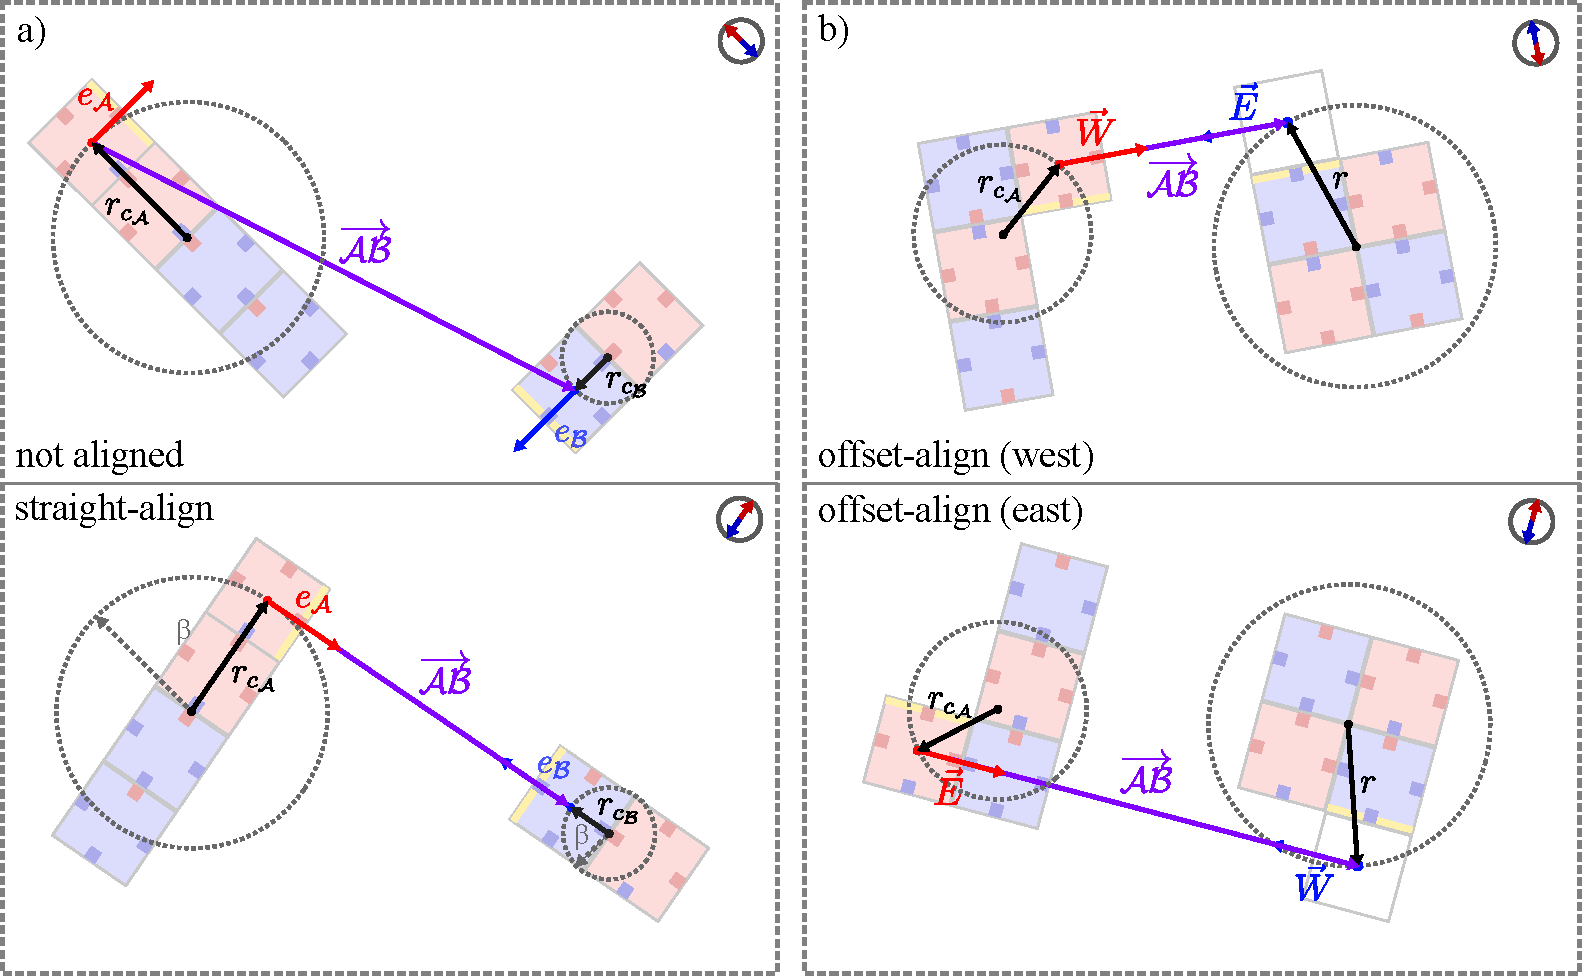
\includegraphics[width=0.90\textwidth]{figures/aligning.pdf}
	\caption[Illustration of straight- and offset-aligning]{The figure shows examples for straight- and offset-aligning. The edges to be connected are marked yellow. a) shows two not aligned polyominoes (top) and the result of a straight-align (bottom). In b) you can see the two approaches for an offset-align. The cubes were aligned with their west edge (top) and with their east edge (bottom).}
	\label{fig:aligning}
\end{figure}

\section{Aligning Cubes}
\label{sec:align}

To establish a connection between two polyominoes $A$ and $B$, the connection-cubes $c_A$ and $c_B$ with their connection-edges $e_A$ and $e_B$ need to be aligned in the correct way.
When $A$ is rotated without magnetic field elevation, a cube with position $P_{c_A}$ rotates in a circle around the center of mass of its polyomino $C_A$.
The vector $\vec{r_A} = P_{c_A} - C_A$ is the radius of this rotation-circle.
When also considering $B$, a rotation of the magnetic field rotates $\vec{r_A}$ and $\vec{r_B}$ by the same angle $\beta$.
The goal is to find this angular difference $\beta$, so that the cubes are aligned.
There are two different approaches for alignment: Straight-align and offset-align.

\paragraph{Straight-Align:}

For straight aligning, we define a vector $\overrightarrow{AB} = P_{c_B} - P_{c_A}$ pointing form $c_A$ to $c_B$.
The aligning is done when $\vec{e_A}$ points in the same direction as $\overrightarrow{AB}$, so $\angle \left( \vec{e_A}, \overrightarrow{AB} \right) = 0$.
Consequently $\angle \left( \vec{e_B}, \overrightarrow{AB} \right) = \pi$, since $e_A$ and $e_B$ have to be opposite edges for a connection.

\autoref{fig:aligning} a) illustrates a straight-align for an east-west connection with all the parameters.
The two polyominoes could now theoretically pivot walk together and connect the desired edges.
Straight-aligning is always used for east-west connections, but we also use it for north-south connection in one special case. More on that in \autoref{sec:plan}.

\paragraph{Offset-Align:}

When considering north-south connections we need to align with an offset, so that the cubes can be moved together from east or west direction.
We again define $\overrightarrow{AB} = \hat{P}_{c_B} - P_{c_A}$ with $\hat{P}_{c_B} = d_o \cdot \vec{e_B} + P_{c_B}$.
We add an offset $d_o$ to $P_{c_B}$ in the direction of $e_B$, so $\overrightarrow{AB}$ points from $P_{c_A}$ to a position above or below $P_{c_B}$.
In a perfect world $d_o = 2 \cdot r_C$ is exactly one cube length, but to avoid failures when moving together, we give the alignment a bigger offset.
Instead of pointing $e_A$ in the same direction as $\overrightarrow{AB}$ we now have two options:
Either solving $\angle \left( \vec{E}, \overrightarrow{AB} \right) = 0$ or $\angle \left( \vec{W}, \overrightarrow{AB} \right) = 0$, depending on if we want to move $A$ in east direction, or in the west direction towards $B$.

You can see the two options for offset-aligning in \autoref{fig:aligning} b).
For the two polyominoes you can also see that aligning with east or west edge can make a difference when moving together.
Establishing a connection by letting $A$ move towards $B$ in west direction is possible, but by moving in east direction other cubes of the polyominoes are blocking the way.
In \autoref{sec:plan} we present a method for checking if moving in from east or west is possible. 

\paragraph{Solving Alignment:}

For calculating angular difference we use the dot-product
\begin{equation*}
\angle (a,b) = \frac{a \cdot b}{\lVert a \rVert \lVert b \rVert} \,,
\end{equation*}
with $a,b \in \mathbb{R}^2$. This way the difference is always positive, which is beneficial in the case of alignment.
We define a function for straight-aligning based on the rotation angle $\beta$, where both $\vec{e_A}$ and $\overrightarrow{AB}$ change according to $\beta$.
\begin{equation}
\delta(\beta) = \angle \left( R_\beta \vec{e_A}, \, \left( R_\beta r_B + C_B \right) - \left( R_\beta r_A + C_A \right)\right) \,.
\end{equation}
$R_\beta$ is a rotation matrix used for rotating vectors by $\beta$.
For an offset-align the function would be
\begin{equation}
\delta(\beta) = \angle \left( R_\beta \vec{e}, \, \left( R_\beta \hat{r_B} + C_B \right) - \left( R_\beta r_A + C_A \right)\right) \,,
\end{equation}
with $\vec{e} \in \{ \vec{E}, \vec{W}\}$ and $\hat{r_B} = \hat{P}_{c_B} - C_B$

Alignment is not always possible, so instead of solving $\delta(\beta) = 0$, we are minimizing $\delta(\beta)$.
Because $-\pi < \beta \leq \pi$ we can iterate through increasing values of $\beta$.
If we encounter a value close enough to zero we can return it.
If not we return the minimum of all the calculated values.
This way we at least get as close to an alignment as possible.

%TODO PLOT of delta(beta) and beta for one example where it gets zero and one where it doesnt. This should further explain why aligning is not always possible

\section{Moving Polyominoes Together}
\label{sec:walk_wait}

Since both polyominoes $A$ and $B$ perform pivot walking motions simultaneously, due to global control, a connection will most likely happen when one polyomino walks into a wall of the workspace boundary.
Connection can only happen in the middle of the workspace when one polyomino is faster than the other, meaning it has a greater pivot walking distance $d_P$.
At a first glance it seems easy to move polyominoes together, after the connection-cubes are aligned as described in \autoref{sec:align}.
The two options of walking left and right determine if either $A$ is chasing $B$, or if $B$ is chasing $A$, which is of course also dependent on their initial position and orientation.
In the end one option might be shorter or better in terms of other polyominoes interfering with $A$ and $B$, but theoretically both are able to establish the connection.

In reality it becomes more difficult.
When a polyomino is continuously walking against a wall at any angle other than 90 degree, the polyomino will move alongside the wall.
In \cite{schmidt2020} research is done on how friction with boundary-walls under global control forces can be used to calculate the necessary motions for reaching a desired goal configuration, but friction forces depend greatly on material choices and are stochastic.
Another difficulty are different orientations of displacement vectors.
It is mathematically possible to calculate the right orientation of the magnetic field to result in a collision after $n$ pivot walking cycle for both polyominoes, even at desired edges, but it is not guaranteed that this collision-point is within the workspace boundaries.
In that case the calculation of friction and displacement have to be combined together with other factors like polyominoes blocking each other or changing their shape during movement.
This is fairly complex and recalculating would be necessary in many situations, so we choose a simpler dynamic approach.

We estimate the pivot walking cycles necessary until $c_A$ moved to the original position of $c_B$, before it is moved with
\begin{equation}
n = \left\lceil \frac{\lVert P_{c_A} - P_{c_B}\rVert}{d_{p,A}} \right\rceil \,.
\end{equation}
We then only walk a portion of $n$ and re-align the cubes.
When $c_A$ and $c_B$ are near enough for magnetic forces to act we frequently wait a short period to let magnetic attraction pull $e_A$ and $e_B$ together.
This will automatically adjust the alignment, but for even more precision we decreased the pivot walking angle $\alpha$ when in close proximity.

\section{Plan and Failures}
\label{sec:plan}

A plan is a sequence of actions $A = a_1, ... , a_n$ that when applied to an initial configuration $g_{init}$, leads to a goal configuration $g_{goal}$.
Two plans can be concatenated when the goal of the first matches with the initial configuration of the second.
That way multiple local plans can be connected to form a global plan.
We define a metric to compare and evaluate plans based on rotational cost of its actions.
We only consider magnetic field rotations, not elevation.
Let $a_i$ be a normal rotation of angle $\beta$, then $\text{cost}(a_i) = |\beta|$.
If it is a pivot walking motion, then $\text{cost}(a_i) = |2\alpha|$.
The cost for the plan is the sum of the costs of all its actions
\begin{equation}
\sum_{i=1}^{n} \text{cost}(a_i) \,.
\end{equation}
A local plan is successful if $g_{goal}$ contains a polyomino with the desired connection of $c_A$ and $c_B$ at $(e_A, e_B)$.
If a plan is successful or not is described by the plan-state $s$.
There are several reasons the local planner might fail to develop a plan:

\paragraph{Impossible Connection:}

Most failures occur, because it is not possible to connect the polyominoes.
First of all, $e_A$ and $e_B$ need to be free, so no other cube is already connected to them, but even if both are free other cubes then $c_A$ and $c_B$ can prevent a connection.
By connecting two polyominoes in one local discrete coordinate-system, for all cubes $c_1$, $c_2$ with coordinates $(x_1, y_1)$, $(x_2, y_2)$: $\left|x_1 - x_2\right| < 1$ and $\left|y_1 - y_2\right| < 1$ should hold true.
If two positions are equal, we call this an overlap, which prevents the connection.
Of course, a connection is never possible if $e_A$ and $e_B$ are part of the same polyomino and not already connected.

All these conditions are easy to check in a discrete way before even starting to plan, but that is not enough.
Connection with other polyominoes during planning can invalidate those pre-checked conditions, so we need to frequently re-check them.

\paragraph{Impossible Slide-In:}

Even if a connection in a common local coordinate-system is possible you can only connect by moving in from east or west.
Other cubes can again prevent this by blocking the way for an easy slide-in.
We can also verify both east and west slide-in in a common local coordinate system.
This discrete check assumes exact movement from east or west direction.
Because of different displacement directions, we know this is not true, but it is a reasonable approximation.
Research on assembling a polyomino out of two parts by moving one part towards the other without collision, was done by Agarwal et al. \cite{agarwal2021}. 

When pre-checking this condition, we can state failure if both directions are not possible.
Otherwise, we can align with respect to the valid slide-in direction, or try out both, if both are possible.
Again, the condition needs to be re-checked frequently, due to changing polyominoes.

\paragraph{Polyominoes being Stuck:}

Polyominoes can get stuck in corners or on walls of the workspace.
In this state it is not possible anymore to decrease the distance of $A$ and $B$ by pivot walking.
We can identify this state when the position of both cubes $c_A$ and $c_B$ do not change after a certain amount of pivot walking motions.

When stuck while trying to establish a north-south connection, a straight-align instead of an offset-align can solve the problem.
It depends on the distance of the cubes after straight-aligning.
If the distance is too big for magnetic forces to act, failure is reported, but if they are close enough the local planner waits until magnetic attraction connects $e_A$ and $e_B$.


\begin{figure}
	\centering
	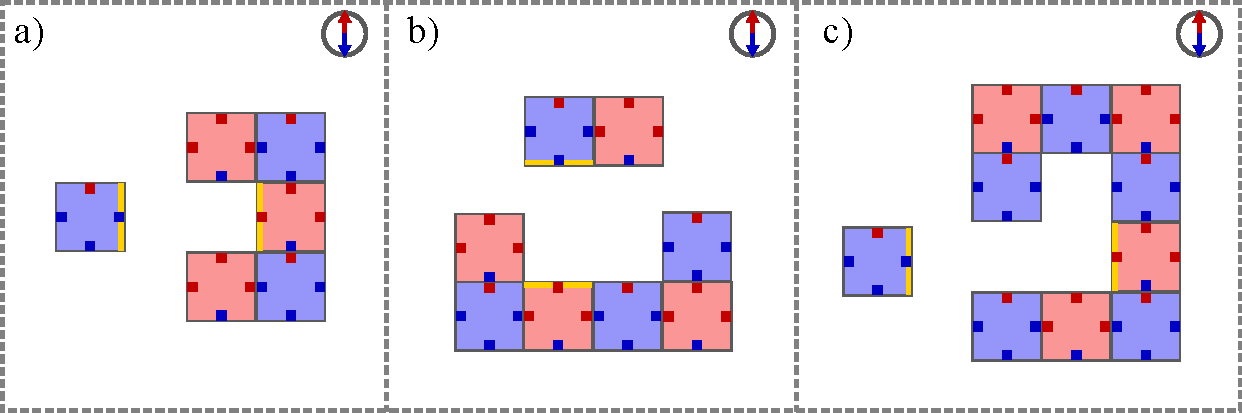
\includegraphics[width=0.80\textwidth]{figures/caves.pdf}
	\caption[Examples for connecting polyominoes into caves]{Three different examples for connecting polyominoes into caves. a) and b) show one-cube-deep caves (a) east-west and b) two-cube-wide north-south). c) illustrates a two-cube-deep east-west cave. The edges to be connected are marked yellow.}
	\label{fig:caves}
\end{figure}

%TODO maybe show bigger caves. Implementation of cave checking still wonky

\paragraph{Connecting in Caves:}

Connecting two polyominoes where one of the connection-faces is located inside a cave is a difficult task in the continuous world.
We differentiate between east-west and north-south located caves.
Furthermore a cave can be of a certain depth and width measured in multiples of $2 r_C$.
\autoref{fig:caves} shows examples for caves with varying depths and widths.

Caves only become problematic when the polyomino to be inserted has the same width as the cave, shown in \autoref{fig:caves} b).
Connecting into a cave with a depth of more than $2 r_C$ is not possible.
For instance, when inserting the blue single cube into the polyomino in \autoref{fig:caves} c), the blue cube would connect with north and south faces of the polyomino before even reaching the full depth of the cave.
But even caves with depth $2 r_C$ are hard to handle.
Inserting into a cave can be done by pivot walking, this would only work for east-west caves, or by letting magnetic forces attract the connection-faces.
Relying on magnetic forces alone seem promising, since it would work for both cave types, but in reality not only the forces of the connection-faces are present.
All the forces between other magnets prevent an easy slide-in.
In our simulator the connection-face will be more attracted or repelled by faces outside the cave, then the once inside.
Pivot walking into east-west caves, even with small values for $\alpha$, has also a high failure rate because of other magnets.
The local planner states failure immediately when polyominoes should be connected in any cave-type.

\paragraph{Invalid Polyominoes:}

Because construction of invalid polyominoes is hard to handle on a global scale, we already omit plans containing them in our local planner.
We state failure if any invalid polyominoes is created at any point during planning.
We also pre-check (and frequently re-check) if the polyomino that will be created by establishing the connection would itself be invalid. 

\paragraph{Maximum Movement Capacity:}

As a worst-case failure, we limit the amount of movement $A$ and $B$ are able to do.
Whenever a pivot walking motion is done, we sum up the distances $c_A$ and $c_B$ moved together.
Let $(w,h)$ be the size of the workspace.
We define a maximum movement capacity of $2\cdot(w+h)$.
This capacity gives the polyominoes enough movement, so that both can move along a horizontal and vertical workspace boundary, which should be sufficient to establish a connection.

\begin{algorithm}
	\caption{\scshape Align-Walk-Realign}
	\label{algo:local_algo}
	\begin{algorithmic}[1]
		\REQUIRE $c_A$, $c_B$, $e_A$, $e_B$, $\vec{w}$, $\vec{m}$, $g_{init}$ 
		\ENSURE $(s, g_{goal}, A)$ \COMMENT{state $s$ and actions $A$ leading to configuration $g_{goal}$}
		\STATE $s \gets \text{undefined}$
		\STATE $g_{goal} \gets g_{init}$
		\STATE $A \gets \{\}$
		\STATE $\text{wait} \gets$ \TRUE
		\LOOP
			\IF[aligning straight or with offset]{$e_A \in \{E,W\}$}
				\STATE $a \gets \text{\scshape Align-Straight}(c_A, c_B, e_A)$
			\ELSE
				\STATE $a \gets \text{\scshape Align-Offset}(c_A, c_B, \vec{m}, e_B)$
			\ENDIF
			\STATE $g_{goal} \gets \text{\scshape Simulate}(g_{goal}, a)$
			\STATE $A \gets \text{\scshape Append}(A, a)$
			\STATE $s \gets \text{\scshape Update-State}(g_{goal}, c_A, c_B, e_A, \vec{m})$
			\IF[first time checking for failure or success]{$s \neq \text{undefined}$}
				\RETURN $(s, g_{goal}, A)$
			\ENDIF
			\IF[wait or walk]{$\text{\scshape Critical-Distance}(c_A, c_B)$ \AND wait}
				\STATE $a \gets \text{\scshape Wait}()$
				\STATE $\text{wait} \gets$ \FALSE
			\ELSE
				\STATE $a \gets \text{\scshape Walk}(c_A, c_B, \vec{w})$ \COMMENT{$a$ can be multiple walking steps (\autoref{sec:walk_wait})}
				\STATE $\text{wait} \gets$ \TRUE
			\ENDIF
			\STATE $g_{goal} \gets \text{\scshape Simulate}(g_{goal}, a)$
			\STATE $A \gets \text{\scshape Append}(A, a)$
			\IF[handle stuck condition]{$\text{\scshape Stuck}(c_A, c_B)$}
				\STATE $a \gets \text{\scshape Align-Straight}(c_A, c_B, e_A)$ \COMMENT{do a straight aligne}
				\STATE $g_{goal} \gets \text{\scshape Simulate}(g_{goal}, a)$
				\STATE $A \gets \text{\scshape Append}(A, a)$
				\WHILE[let magnets attract until stuck again]{\NOT $\text{\scshape Stuck}(c_A, c_B)$}
					\STATE $a \gets \text{\scshape Wait}()$
					\STATE $g_{goal} \gets \text{\scshape Simulate}(g_{goal}, a)$
					\STATE $A \gets \text{\scshape Append}(A, a)$
				\ENDWHILE
			\ENDIF
			\STATE $s \gets \text{\scshape Update-State}(g_{goal}, c_A, c_B, e_A, \vec{m})$
			\IF[second time checking for failure or success]{$s \neq \text{undefined}$}
				\RETURN $(s, g_{goal}, A)$
			\ENDIF
		\ENDLOOP 
	\end{algorithmic}
\end{algorithm}

\section{Local Planning Algorithm}
\label{sec:local_algo}

Before executing the algorithm presented in \autoref{algo:local_algo} we evaluate all the failure conditions that can be checked in advance, so no simulation-time is wasted on a plan that is bound to fail from the start.
While doing so, the possible slide-in directions are also determined and \autoref{algo:local_algo} is executed with both pivot walking directions $\vec{w}$ for each possible $\vec{m}$.
This means for an east-west connection, we always develop two plans and for a north-south connection two or four, depending on the slide-in directions.

In the end, the successful plan with the lowest costs is returned.
Even if all plans fail, we still determine the best failure.
Again, plans with lower costs are preferable, but we favor impossible connection and slide-in failures.
These failures just state that we can not establish a specific connection, but a global planner could continue to plan based on the goal configuration the local planner ended in.
A configuration when the polyominoes are stuck, or the maximum movement capacity is reached, is not good for further planning, but invalid polyominoes or polyominoes with caves will definitely be omitted on a global scale.

The different plans are developed in parallel and if one process finishes with a successful plan, the execution of all other plans can be canceled.
This saves a lot of computation time, although we might not return the best plan, since fastest computation does not automatically mean lowest costs.
Generally speaking a low computation time can be linked with low rotational cost, because the local planner spends the majority of time, about $98\%$, on simulating the actions.

\paragraph{Align-Walk-Realign:}

\autoref{algo:local_algo} takes the connection-cubes and edges $c_A$, $c_B$, $e_A$, $e_B$ along with $\vec{w}$, $\vec{m}$ and an initial configuration $g_{init}$ as inputs and returns a plan-state $s$ along with the configuration $g_{goal}$ the algorithm ended in after applying the sequence of actions $A$.
The algorithm runs in a loop until $s$ changes to success or one of the failure condition.
The failure and success conditions are evaluated twice per iteration with {\scshape Update-State}.
Once after aligning, and once at the end of the loop.
That way, the planner avoids simulating unnecessary actions.
$g_{goal}$ is updated by simulating the determined actions with {\scshape Simulate}.
The actions are appended to $A$ after simulation.
We perform either a straight or offset-align, depending on $e_A$ and $e_B$.
The offset-align is done with the direction of $\vec{m}$.
After aligning we walk the estimated amount of pivot walking cycles (\autoref{sec:walk_wait}) in direction $\vec{w}$ with {\scshape Walk}, or we wait with {\scshape Wait}, if $c_A$ and $c_B$ are in close proximity, determined by {\scshape Critical-Distance}.
If we waited in the previous iteration, we walk in the current one and oppositely.
This behavior is toggled by the variable $wait$. 
The stuck condition is evaluated with {\scshape Stuck} and does not state failure immediately, since a straight-align might be able to fix the situation.
When the polyominoes are stuck, the algorithm performs a straight-align and waits as long as this changes the stuck condition.

\subsection{Complexity}
\label{sec:local_complex}

\paragraph{Optimality}

In our case the optimal plan for connecting two polyominoes is the one establishing the connection with the lowest rotational cost, as defined in \autoref{sec:plan}.
We use this metric, because it is strongly linked with computation time, but can also be interpreted in a real word application of modular magnetic cubes.
Even if the local planner would not calculate plans in parallel, our dynamic approach of realigning does not produce optimal solutions.
It therefore simulates only the actions that are included in the final plan, which minimizes simulation time.

Optimality could be archived, when sliding on walls and different polyomino displacements, as described in \autoref{sec:walk_wait}, are not existent.
It is easy to see that after aligning, both pivot walking directions produce plans that move the polyominoes together in a straight path.
The plan with the shorter path would be optimal is this theoretical case.
But these factors have to be considered, and even if they were by a local planner it is hard to say, if that would be enough to actually prove optimality.

\paragraph{Completeness}

The local planner is also no complete.
Just because the up to four plans it evaluates fail, does not prove the non existence of a action sequence that would establish the desired connection.
If other polyominoes are blocking the way of $A$ and $B$, complex movements around these polyominoes, instead of the more or less straight path we are taking, could create solutions where our planner fails.
The reason we choose this simple approach is again to avoid simulation as much as possible. 


%TODO comic sequence FIGURE of the algorithm






